%!TEX root = ../../../memoria.tex

\section{Productos}

	\subsection{Vista global de productos}\label{chapter:section:productos:subsection:vista_global}
		La interfaz inicial de la aplicación corresponde a la vista de todos los productos que el sistema tiene. En la \refFigura{figure:solution:product:global_view:view} se pueden observar 4 productos.

		\begin{figure}[H]
			\centering
			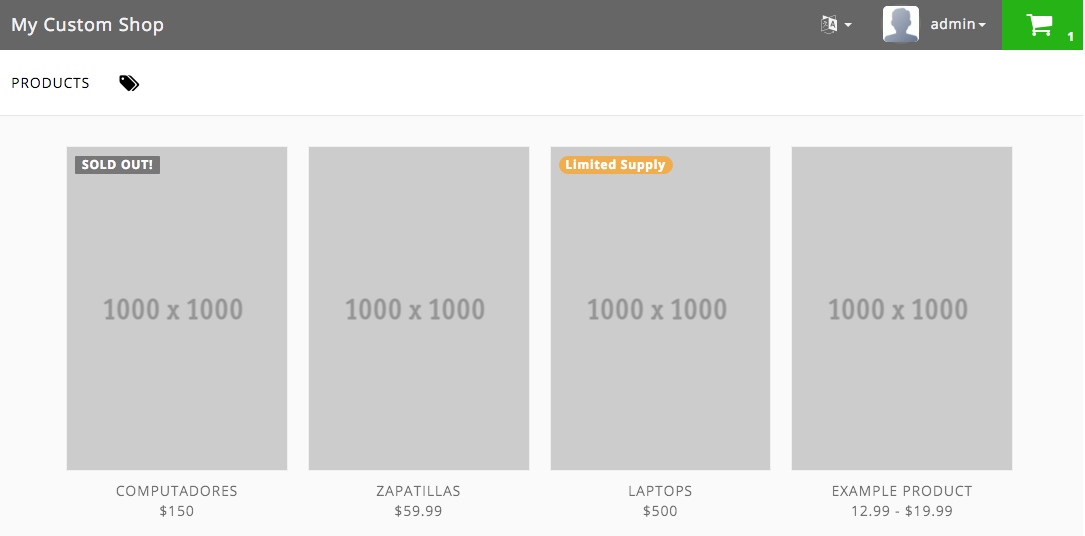
\includegraphics[width=0.8\textwidth]{figuras/solution/product/global_view/view.png}

			\caption{Vista global de los productos. Productos con problemas de \stock dan información.}
			\label{figure:solution:product:global_view:view}
		\end{figure}

		De la interfaz, se observa que hay un producto \textit{SOLD OUT!} y otro producto \textit{LIMITED SUPPLY}. Esto ocurre por que la plataforma tiene un sistema de \trackingCPT de productos la cual puede ser modificada desde la vista \nameref{chapter:section:productos:subsection:edicion}.


		Esta vista depende de los permisos que el usuario que ha ingresado tiene. Si el usuario tiene permisos de edición de productos, tendra la posibilidad de ver todos los productos que existen en el sistema, incluso esos que no estan publicados. En el caso de un usaurio sin permisos de edición, solo tendrá visibilidad de aquellos productos que han sido publicados.

	\subsection{Descripción de un producto}\label{chapter:section:productos:subsection:descripcion}

		La aplicación permite consultar la descripción de un producto. Dicha interfaz puede observarse en la \refFigura{figure:bootstrap:theme_cyborg}. Se puede aprenciar algunas de las carecterísticas de las que ya dispone cada producto.

		\begin{itemize}
			\item
				Un título del producto.
			\item
				Un subtítulo para dar un resumen.
			\item
				Un espacio para la foto del producto.
			\item
				Un lugar para la descripción del producto.
			\item
				Un precio ó intervalo de precios.
		\end{itemize}

	\subsection{Creación de un producto}

		Cuando se penso en la interfaz de creación/edición de un producto, la base era tener una interfaz idéntica a la vista de \nameref{chapter:section:productos:subsection:descripcion}, y por lo tanto, interactuar con los diferentes elementos directamente en la interfaz de vista.
		Cuando se ingresa a la interfaz de vista de un producto con los pemisos adecuados, todas las componenetes de la vista del producto se vuelven componentes editables.

		La interfaz de creación de un producto se observa en la \refFigura{figure:solution:product:create:form}. Es importante destacar la ayuda que brindan los \placeholdersINT para guiar al usuario.

		\begin{figure}[H]
			\centering
			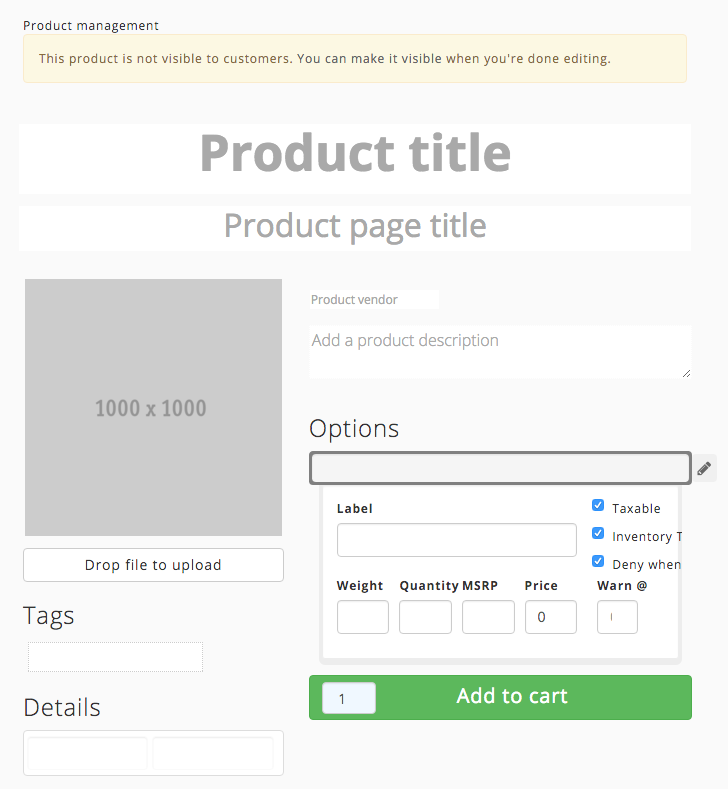
\includegraphics[width=0.8\textwidth]{figuras/solution/product/create/form.png}

			\caption{Interfaz de creación de un producto.}
			\label{figure:solution:product:create:form}
		\end{figure}

		De los campos que se observan en la \refFigura{figure:solution:product:create:form}: \titleForm, \pageTitleForm, \vendorForm, \descriptionForm, \tagsForm y \detailsForm, tienen \feedbackReactivoDEF. Las restricciones en la creación de un producto se encuentra en la \reftabla{tab:solution:products:create:form:product:generic}. 

		\begin{table}[H]
		    \centering
			\begin{tabular}{ |l|c||l| }
				\hline Campo & Requerido & Restricción \\ \hline
				\multirow{1}{*}{\titleForm} 			&  \multirow{1}{*}{\checkmark} & - Debe tener al menos un caracter. \\ \hline
				\multirow{1}{*}{\pageTitleForm} 	&  \multirow{1}{*}{} &  \\ \hline
				\multirow{1}{*}{\vendorForm}		&  \multirow{1}{*}{} &  \\ \hline
				\multirow{1}{*}{\optionsForm}		&  \multirow{1}{*}{\checkmark} &  \\ \hline
				\multirow{1}{*}{\descriptionForm}	&  \multirow{1}{*}{} &  \\ \hline
				\multirow{1}{*}{\multimediaForm}	&  \multirow{1}{*}{} &  \\ \hline
				\multirow{1}{*}{\tagsForm}			&  \multirow{1}{*}{} &  \\ \hline
				\multirow{1}{*}{\detailsForm}		&  \multirow{1}{*}{} &  \\ \hline
			\end{tabular}
		 	\caption{Resumen restrincciones para formulario creación de un producto.}
		    \label{tab:solution:products:create:form:product:generic}
		\end{table}

		Como se aprecia en la \reftabla{tab:solution:products:create:form:product:generic}, el campo \detailsForm no es requerido, sin embargo, cada \detailForm en realidad es un objeto compuesto cuyos campos si son obligatorios(\reftabla{tab:solution:products:create:form:product:generic:details}).
		\begin{table}[H]
		    \centering
			\begin{tabular}{ |l|c||l| }
				\hline Campo & Requerido & Restricción \\ \hline
				\multirow{1}{*}{\textit{Anónimo key}}	&  \multirow{1}{*}{\checkmark} & - Debe tener al menos un caracter. \\ \hline
				\multirow{1}{*}{\textit{Anónimo Value}}	&  \multirow{1}{*}{\checkmark} & - Debe tener al menos un caracter. \\ \hline
			\end{tabular}
		 	\caption{Resumen restrincciones para formulario creación de \detailsForm.}
		    \label{tab:solution:products:create:form:product:generic:details}
		\end{table}

		\begin{table}[H] 
		    \centering
			\begin{tabular}{ |l|c||l| }
				\hline Campo & Requerido & Restricción \\ \hline
				\multirow{1}{*}{\textit{Label}}		&  \multirow{1}{*}{\checkmark} 	& - Debe tener al menos un caracter \\ \hline
				\multirow{1}{*}{\textit{Weight}}	&  \multirow{1}{*}{\checkmark} 	& - Número racional mayor o igual a '0' \\ \hline
				\multirow{1}{*}{\quantityForm}	&  \multirow{1}{*}{\checkmark} 	& - Número entero \\ \hline
				\multirow{1}{*}{\msrpSIGLAS}		&  \multirow{1}{*}{} 			& - Número racional mayor o igual a '0' \\ \hline
				\multirow{1}{*}{\priceForm}		&  \multirow{1}{*}{\checkmark} 	& - Número racional mayor o igual a '0' \\ \hline
				\multirow{1}{*}{\denyForm}		&  \multirow{1}{*}{\checkmark} 	& - Boolean \\ \hline
				\multirow{1}{*}{\warnForm}		&  \multirow{1}{*}{} 			& - Número racional mayor o igual a '0' \\ \hline
				\multirow{1}{*}{\taxableForm}	&  \multirow{1}{*}{\checkmark} 	& - Boolean \\ \hline
				\multirow{1}{*}{\trackingForm}	&  \multirow{1}{*}{\checkmark} 	& - Boolean \\ \hline
			\end{tabular}
		 	\caption{Resumen restrincciones para formulario creación de \optionsForm.}
		    \label{tab:solution:products:create:form:product:generic:options}
		\end{table}

	\subsection{Edición de un producto}\label{chapter:section:productos:subsection:edicion}

		Al igual que para la creación de productos, la edición requiere de permisos especiales. Si se cuenta con dichos permisos especiales, la interfaz de la vista de un producto inmediatamente permite editar los campos. Para editarlos, simplemente es necesario seleccionar la componente con el \mousePC y hacer un \click. La componente cambiara su aspecto para dar \feedback al usuario de que esta seleccionada dicha componente y que puede realizar sobre el ediciones. En la \refFigura{figure:features:interfaz_edicion_editando_description} y \ref{figure:features:interfaz_edicion_editando_subtitulo} es posible apreciar la componenete que se ha seleccionado para editar.

		\begin{figure}[H]
			\centering
			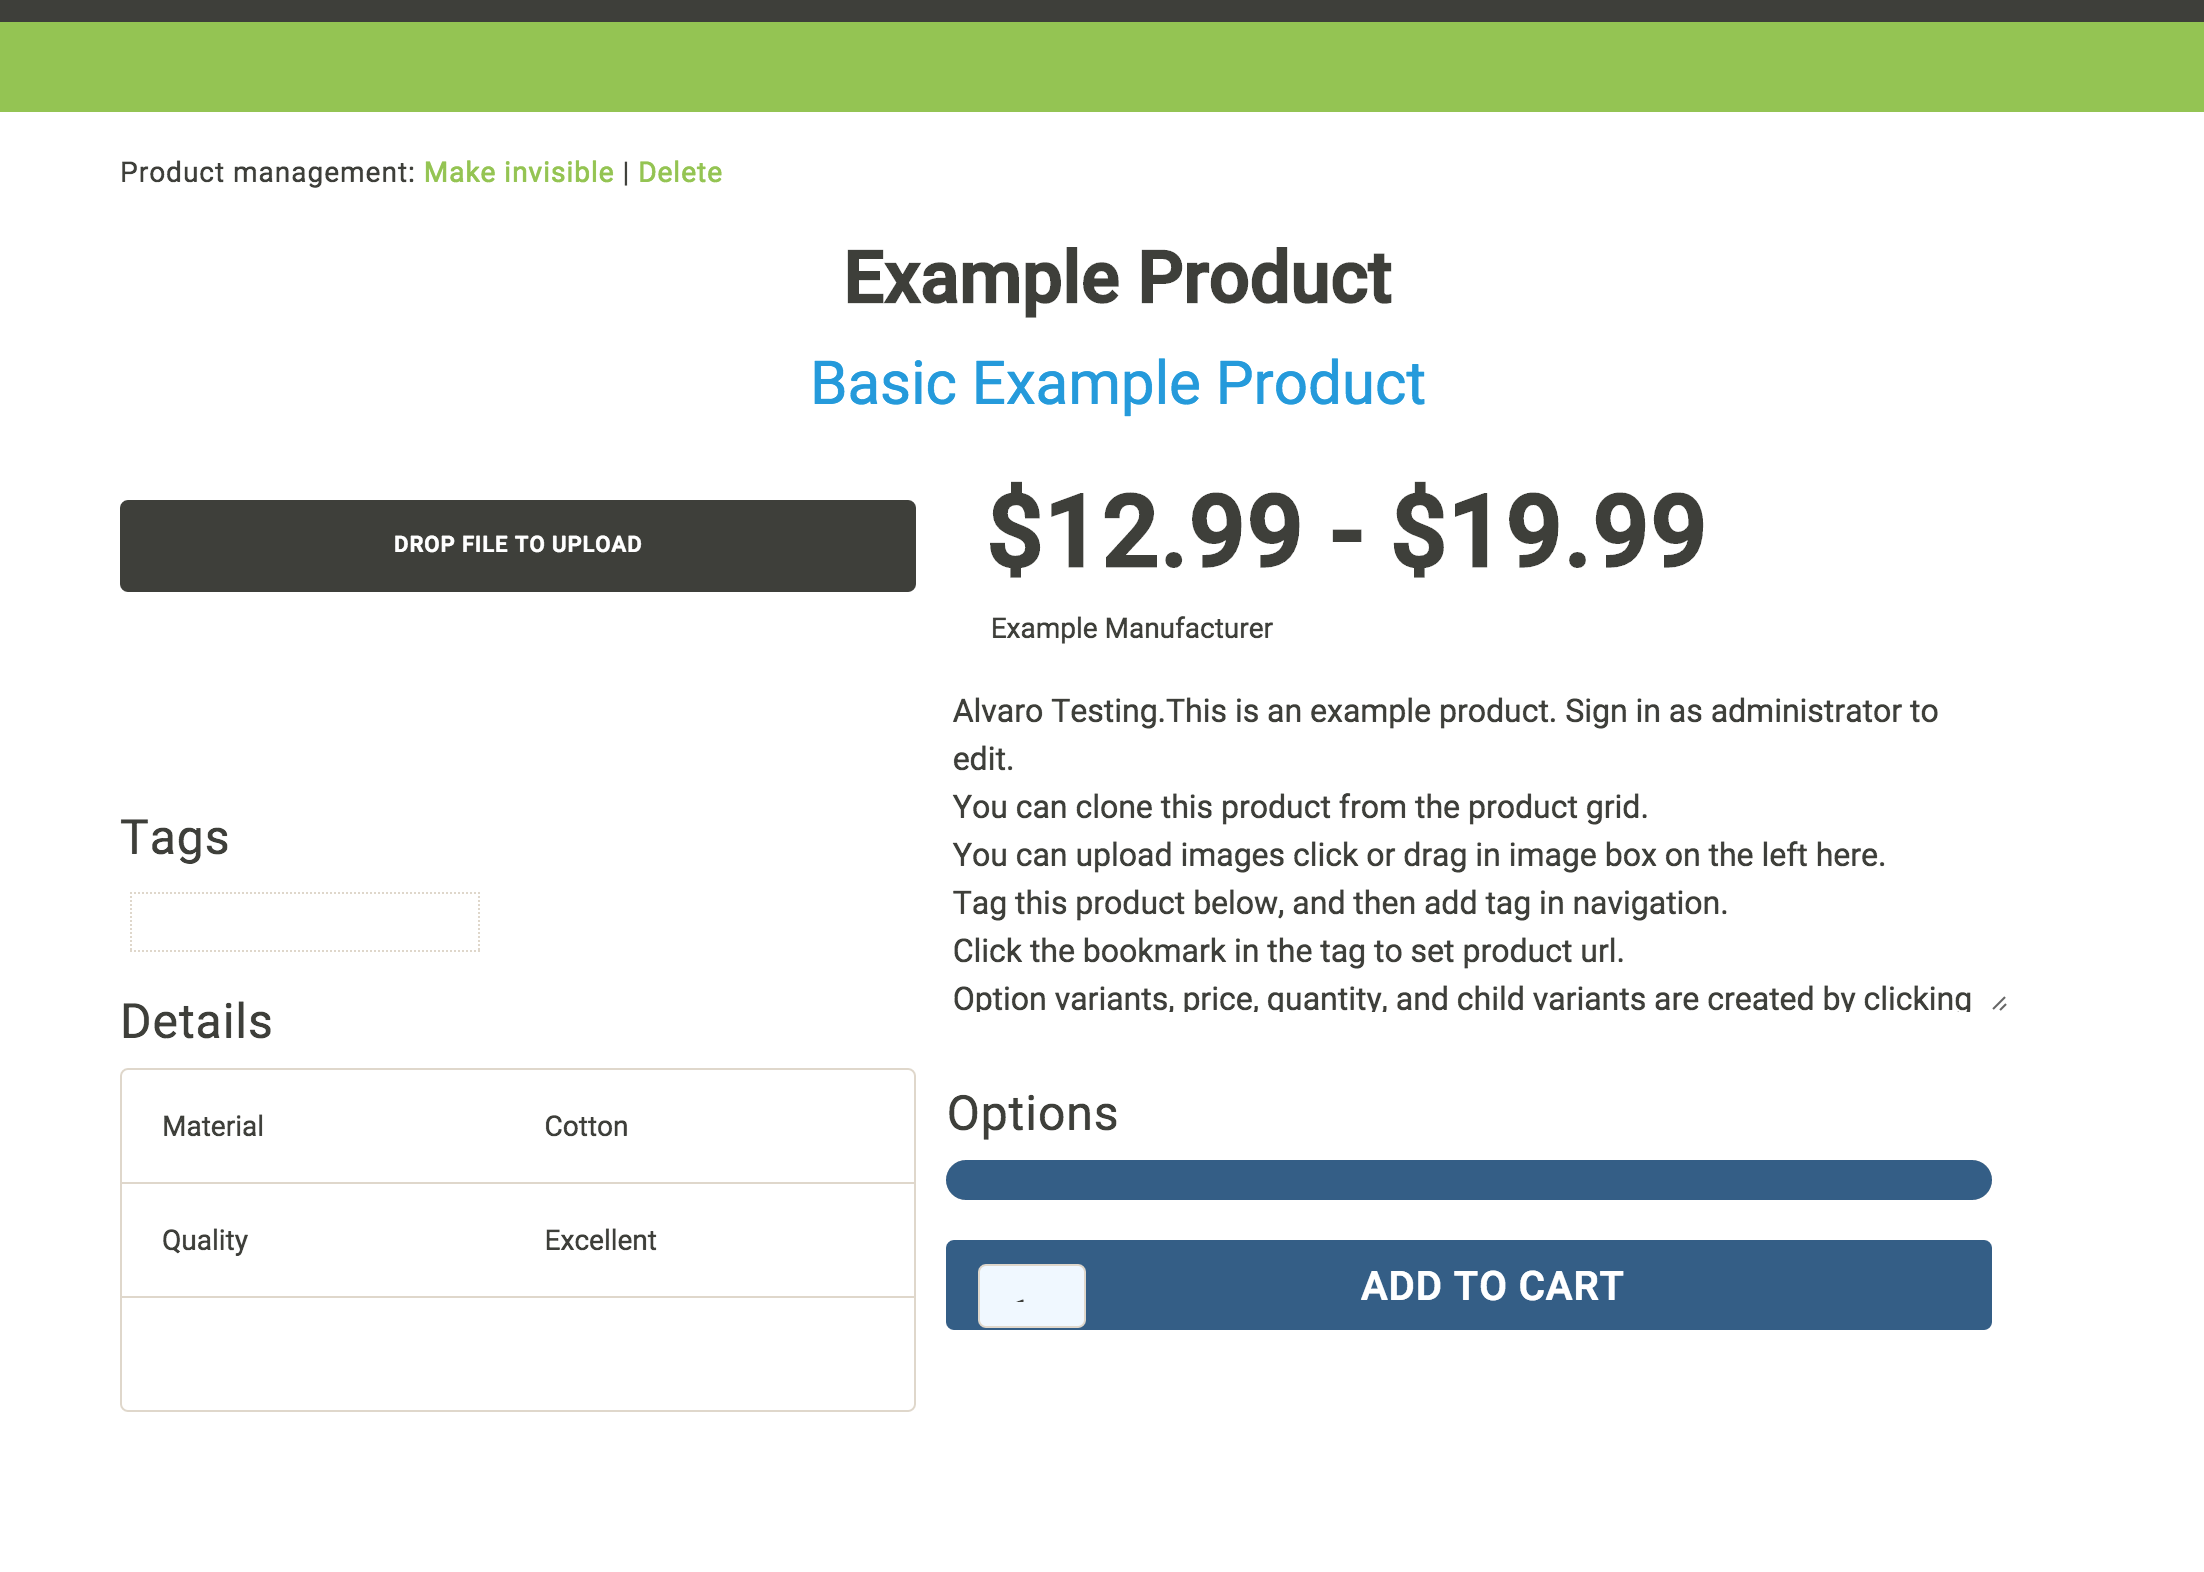
\includegraphics[width=0.8\textwidth]{figuras/productos/interfaz_edicion_producto.png}

			\caption{Interfaz de la edición de un producto.}
			\label{figure:features:interfaz_edicion_producto}
		\end{figure}

		\begin{figure}[H]
			\centering
			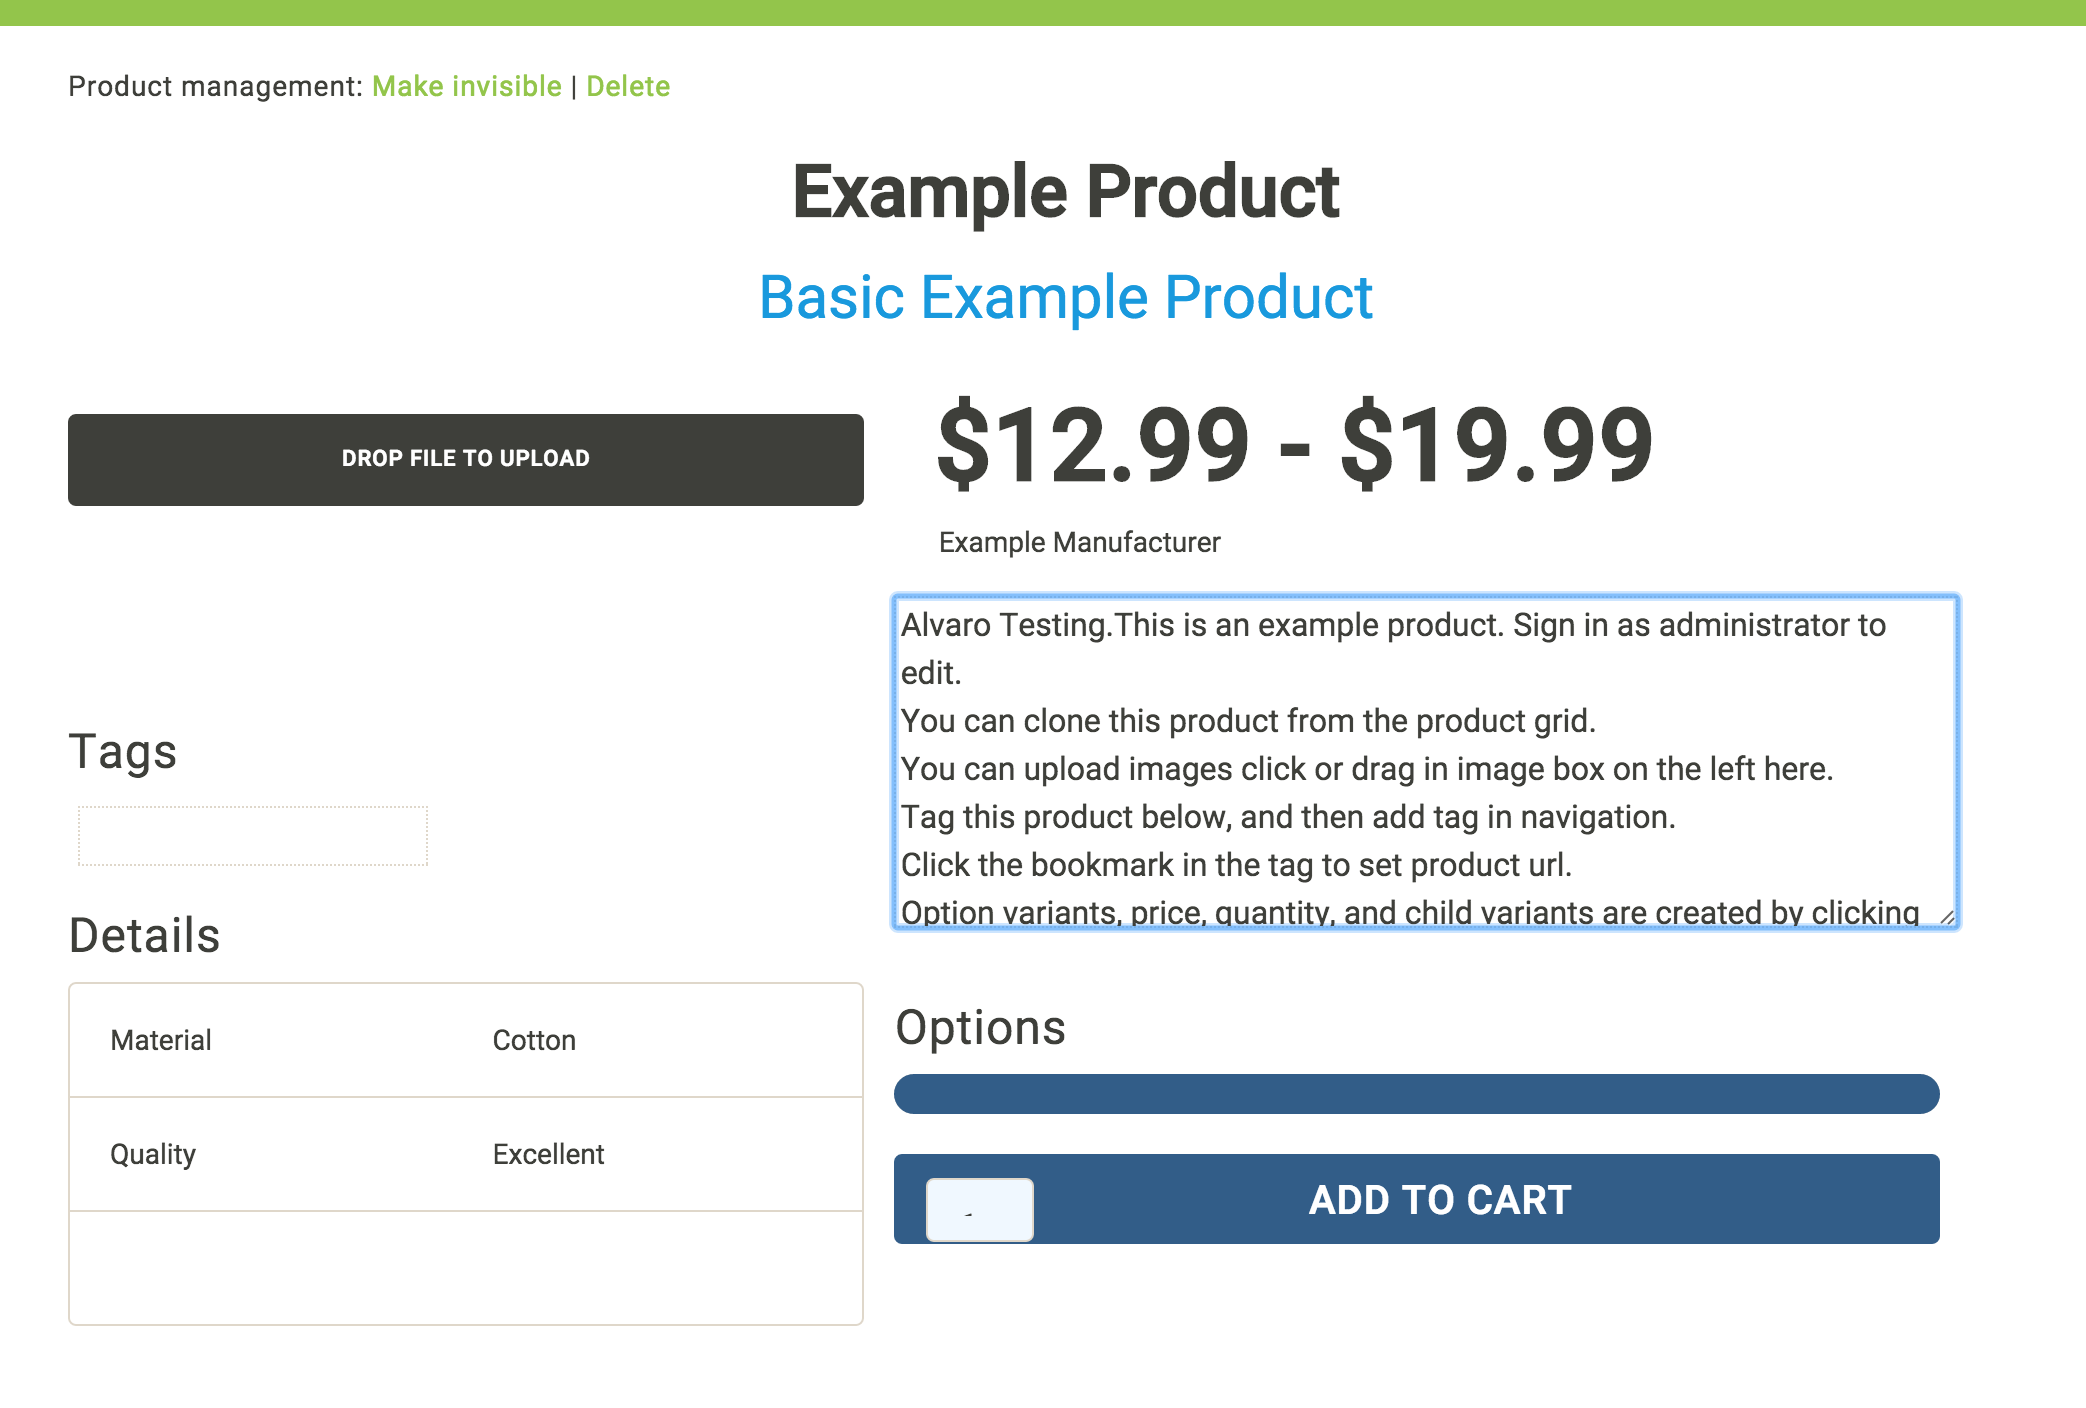
\includegraphics[width=0.8\textwidth]{figuras/productos/interfaz_edicion_editando_description.png}

			\caption{Campo descripción seleccionado para edición.}
			\label{figure:features:interfaz_edicion_editando_description}
		\end{figure}


		\begin{figure}[H]
			\centering
			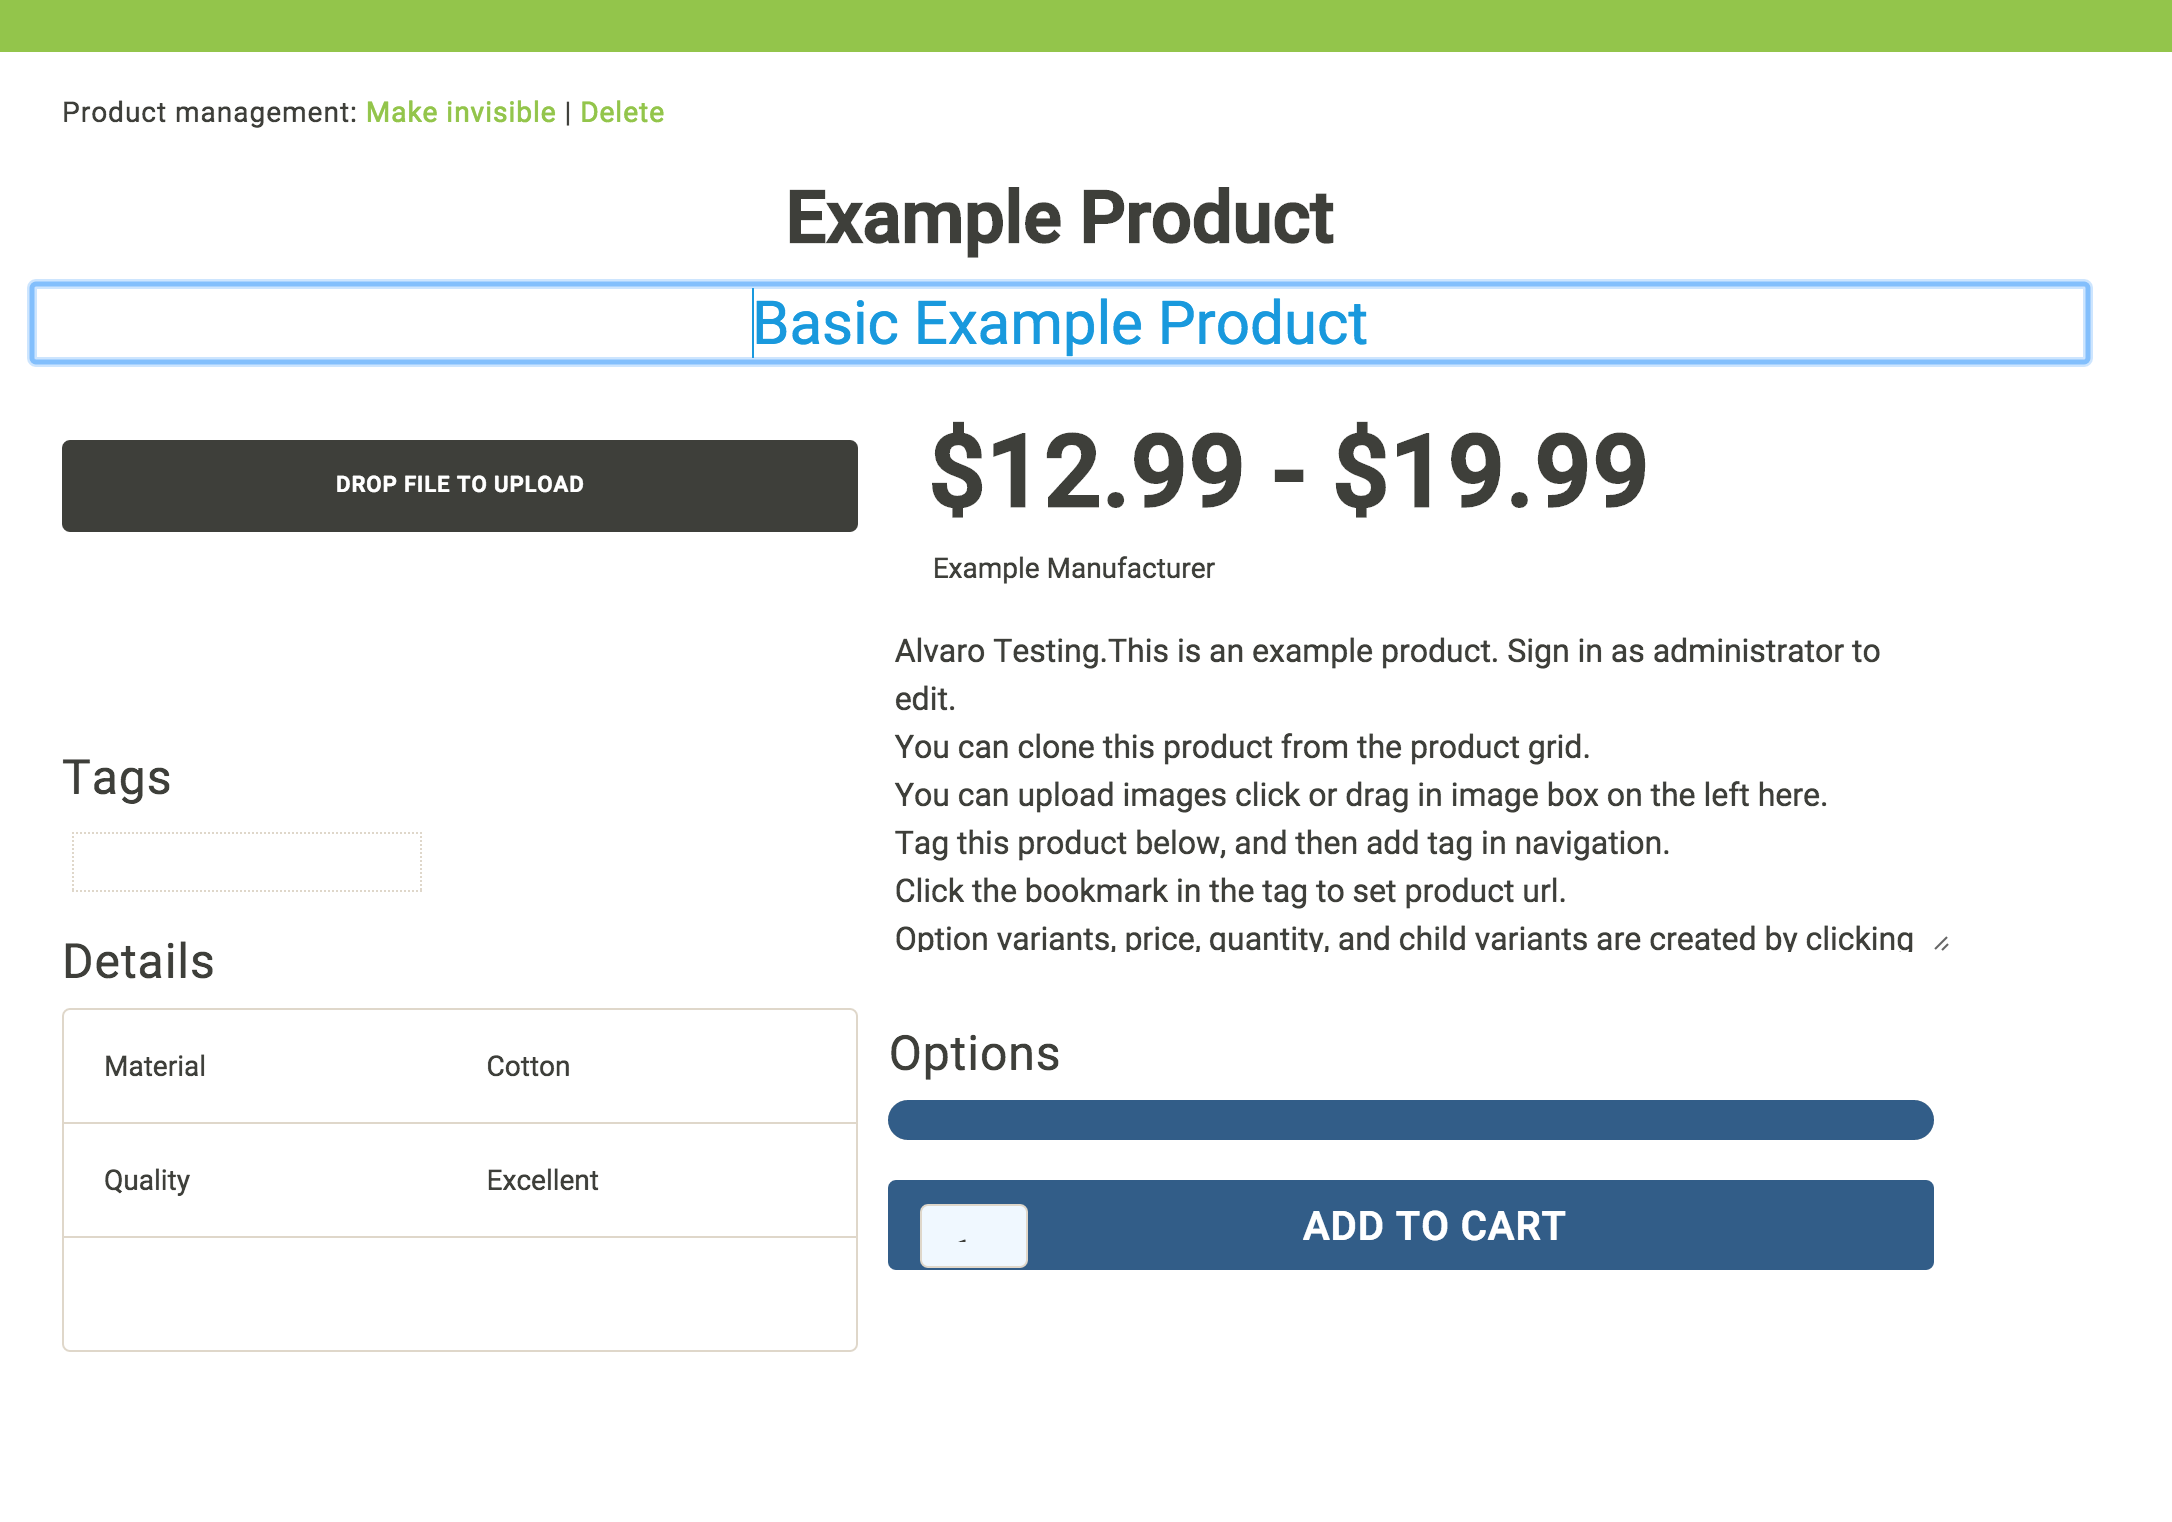
\includegraphics[width=0.8\textwidth]{figuras/productos/interfaz_edicion_editando_subtitulo.png}

			\caption{Campo subtítulo seleccionado para edición.}
			\label{figure:features:interfaz_edicion_editando_subtitulo}
		\end{figure}

		Es importante mencionar que la edición de producto es \reactive, por lo tanto todos los cambios que se realizen serán inmediatamente visibles por parte de todos los usuarios que esten mirando la descripción del producto incluso sin la necesidad de que el usuario haga un \refreshCPT del \websiteINT.

	%TODO: Agregar esta seccion en el futuro
	%\subsection{Eliminación de un producto}

	\subsection{Visibilidad de un producto}

		Todo producto válido puede ser visible para todos los usuarios(visibilidad global), o solo visible para aquellos que tienen permiso de edición sobre dicho producto. En la \refFigura{figure:solution:product:visibility:new} se ve el caso particular de un producto que esta en proceso de creación (no tiene título, el cual es requerido).

		\begin{figure}[H]
			\centering
			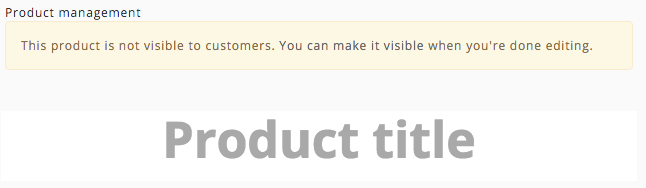
\includegraphics[width=0.8\textwidth]{figuras/solution/product/visibility/new.png}

			\caption{Producto con visibilidad limitada. Además no tiene título.}
			\label{figure:solution:product:visibility:new}
		\end{figure}

		Después de llenar todos los campos mínimos requeridos para la creación de un producto, es posible presionar el \linkINT \youCanMakeItVisibleLABEL y dar visibilidad global al producto. En el caso que no estén llenos todos los campos requerídos, entonces se generá un \autoFocoINT del primer campo no completado requerido. Suponiendo que se intenta dar visibilidad del producto de la \refFigura{figure:solution:product:visibility:new}, se hara un \autoFocoINT del campo título, el cual puede observarse en la \refFigura{figure:solution:product:visibility:autofocus}; además de mantener el estado de visibilidad (no visible para todos). Esto ocurre para mostrar claramente al usuario que esta sucediendo \cite{online_google_ui_pattern_error,online_goodgui_org}.

		\begin{figure}[H]
			\centering
			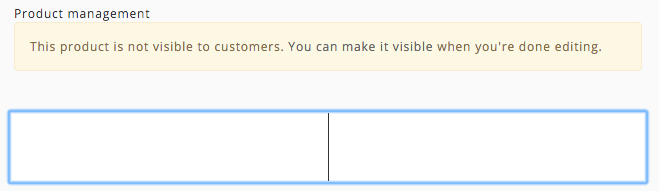
\includegraphics[width=0.8\textwidth]{figuras/solution/product/visibility/autofocus.png}

			\caption{Resultado tras dar visibilidad a un producto sin título. Se genera un \autoFocoINT en el campo título, dado que este es requerido y el estado de visibilidad del producto continua igual.}
			\label{figure:solution:product:visibility:autofocus}
		\end{figure}

		Si todos los campos requeridos de un producto están completos, y se presiona el \linkINT \youCanMakeItVisibleLABEL, se tendra el resultado de la \refFigura{figure:solution:product:visibility:global_visibility}; en donde se observa como el texto superior cambío. Ahora aparece un \linkINT con el texto \makeInvisibleLABEL, para dar \feedback al usuario de lo que ha ocurrido \cite{online_google_ui_design_material,online_goodgui_org}.

		\begin{figure}[H]
			\centering
			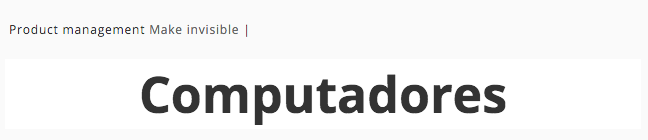
\includegraphics[width=0.8\textwidth]{figuras/solution/product/visibility/global_visibility.png}

			\caption{Producto con visibilidad global. Aparece un \linkINT \makeInvisibleLABEL para ocultar el producto.}
			\label{figure:solution:product:visibility:global_visibility}
		\end{figure}

		%Si se intenta dar visibilidad global de un producto que no esta completo (ver requerimientos de \reftabla{tab:solution:products:create:form:product:generic}), se hará un autofoco al primer elmemento que sea requerido pero que no este completo. Como ejemplo, vemos la \refFigura{figure:solution:product:visibility:new} 	
